\section{Three ways of looking at the state of play}

%This is the new section 2.1

Roads are “congested” when the number of vehicles using them causes unacceptable levels of discomfort and delay. But of course “unacceptable” means different things to different people. Three different perspectives – those of motorists, engineers, and economists – provide definitions that can help policy-makers. 

For motorists, a road is too congested if their speeds drop too far and their trip takes too much longer than expected. Expected travel time is depends on location, time of day, and type of road. The main way to assess congestion from the motorist's perspective is to compare travel times when there is congestion with travel times for the same trip when there is no congestion – usually in the middle of the night. This measure is useful for policy-makers only when comparing congestion across cities of similar sizes. This is because the economic cost of congestion depends on the size of the city.

Traffic engineers consider a road congested when more vehicles are attempting to use the road than it has physical capacity to carry. Capacity refers to the maximum number of vehicles the road is capable of carrying over a fixed period – the maximum possible throughput.

Economists focus on the costs and benefits that road users experience at different levels of traffic flow. They pay particular attention to the difference between the private cost of an additional trip and the social cost of that trip. \Vref{box:explaining-congestion-as-negative-externality} explains how these two concepts can differ, creating the social costs of congestion. 

\Vref{chap:appendix-defining-congestion} provides more detail about each of these definitions. The following sections of this chapter use each to develop an insight into the state of play of congestion in Australia in 2017. 





\section{Engineers will tell you that few roads are congestion beyond their physical capacity}\label{subsec:quantifying-capacity}

%This is the text to be the new section 2.3, i.e. to replace the existing section 3.2 

Engineers' concerns are with the flows of traffic and the carrying capacity of the roads.
On these grounds, they will tell you there is not much cause for concern.

Engineers measure a road's Level of Service (or LOS) on a scale from A to F, where A is free-flowing traffic and F is flow breakdown.%
    \footcite[][Part~3: Traffic Studies and Analysis, p.~63]{Austroads-2015-Guide-Traffic-Mgmt}

On this measure, Sydney and Melbourne's arterial roads generally perform well. Even in some of the most congested inner-suburban corridors, travel flow is, on average, very good for most of the time on an average day
(see \Vref{fig:LOS-innersuburb-SYD}).

Even on the worst weekday in a typical week, peak-hour traffic flows are stable, with most roads providing a LOS better than D,%
    \footnote{``Level of Service D indicates a less stable condition in which small increases in flow may cause substantial increases in delay and decreases in travel speed\dots{} The travel speed is between 40\% and 50\% of the base free-flow speed'': \textcite[][Part~3, p.~63]{Austroads-2015-Guide-Traffic-Mgmt}.}
although the chart shows that flows do become unstable at times, which can be seen here on particularly congested routes in Melbourne.


\begin{figure*}
\begin{minipage}[t][\textheight]{\columnwidth}
    \captionsetup{oneside, margin={0em,-10em}}
	\caption{The average level of service on a selection of short routes in Sydney and Melbourne}\label{fig:LOS-innersuburb-SYD}
	\units{Travel speed as a proportion of free-flow travel speed, and level of service category}
	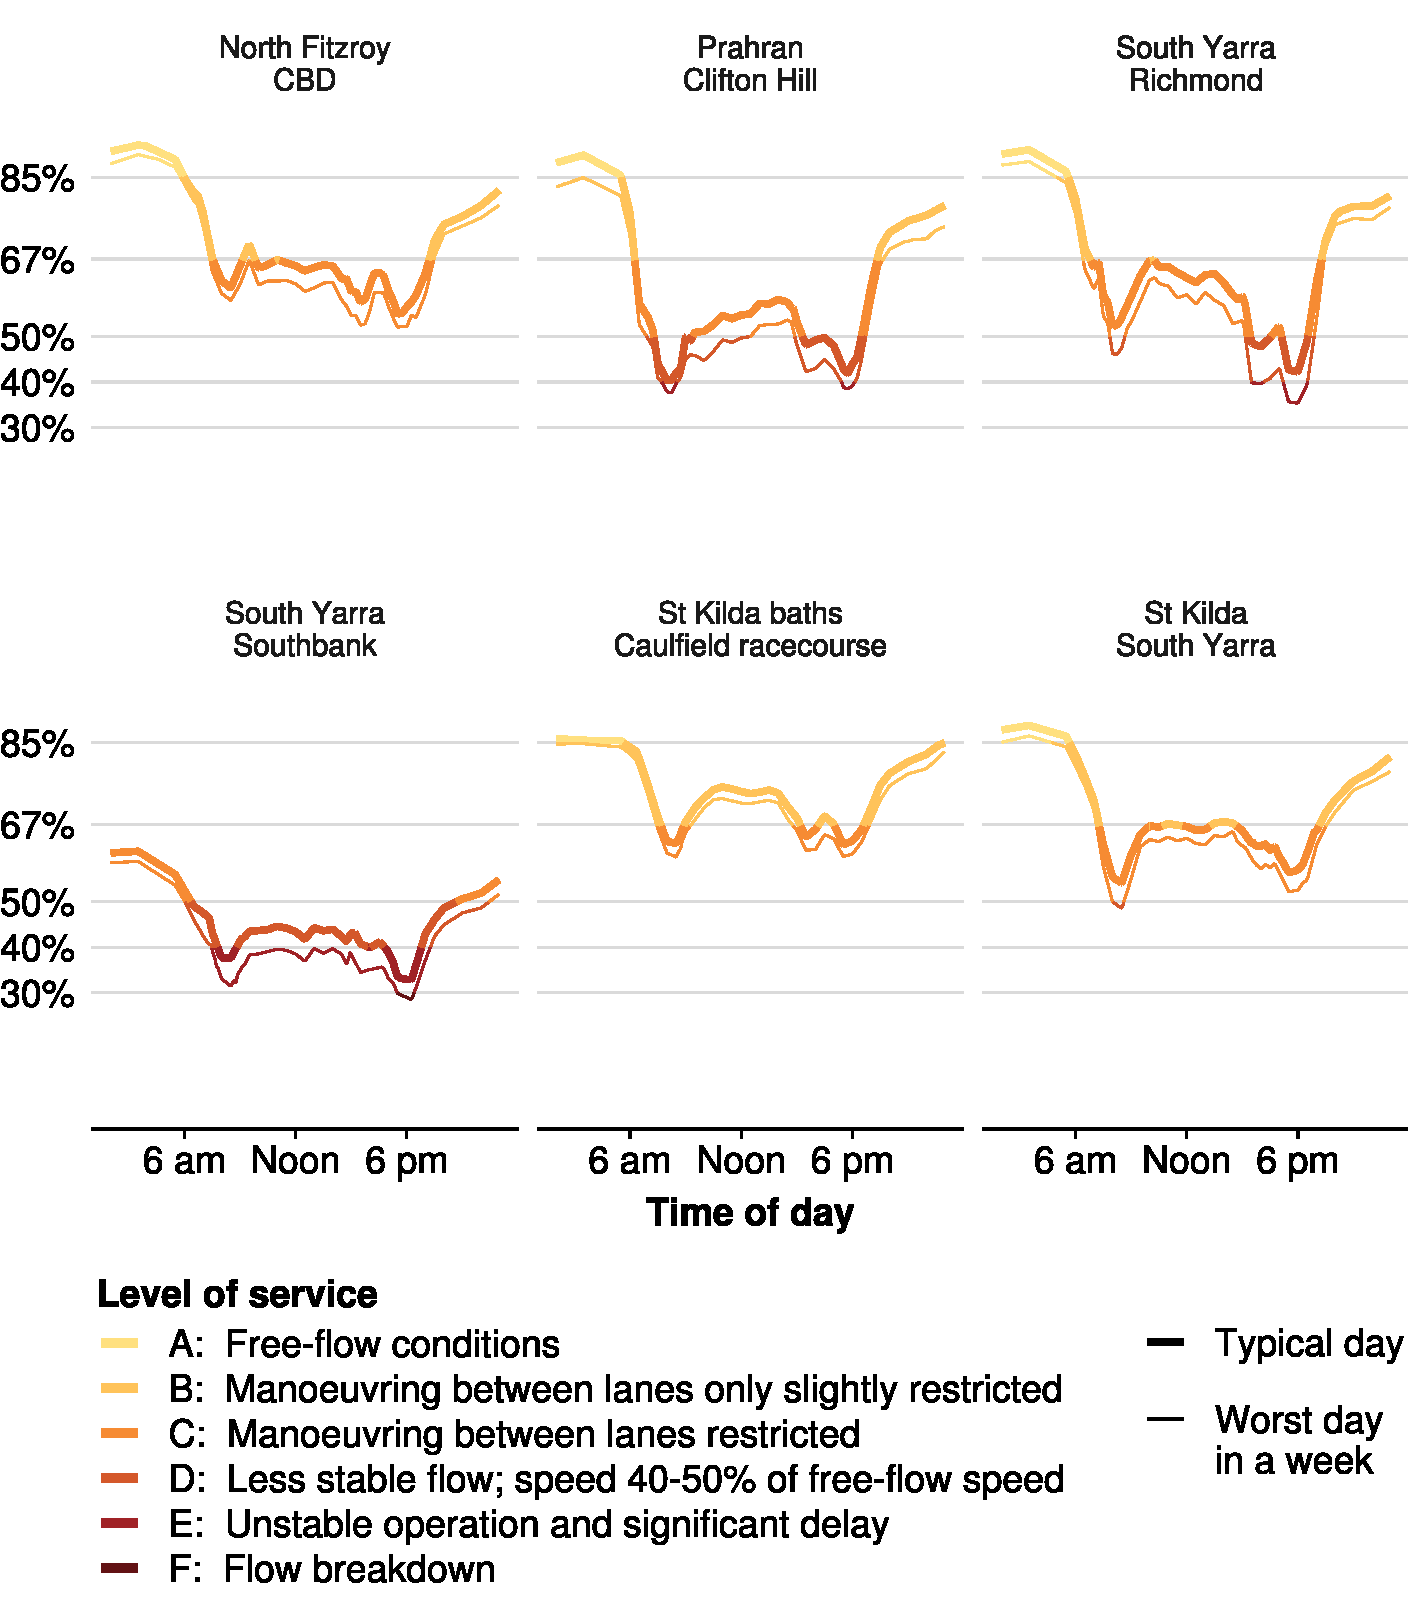
\includegraphics[width=1.06\columnwidth]{atlas/Avg-LOS-short-routes-MEL-1.pdf}
	\sources{Grattan analysis of Google Maps, and \textcite[][Part~3: Traffic Studies and Analysis]{Austroads-2015-Guide-Traffic-Mgmt}}
\end{minipage}
\hfill
\begin{minipage}[t][\textheight]{\columnwidth}
  \caption*{\null}
  \units{\null}
  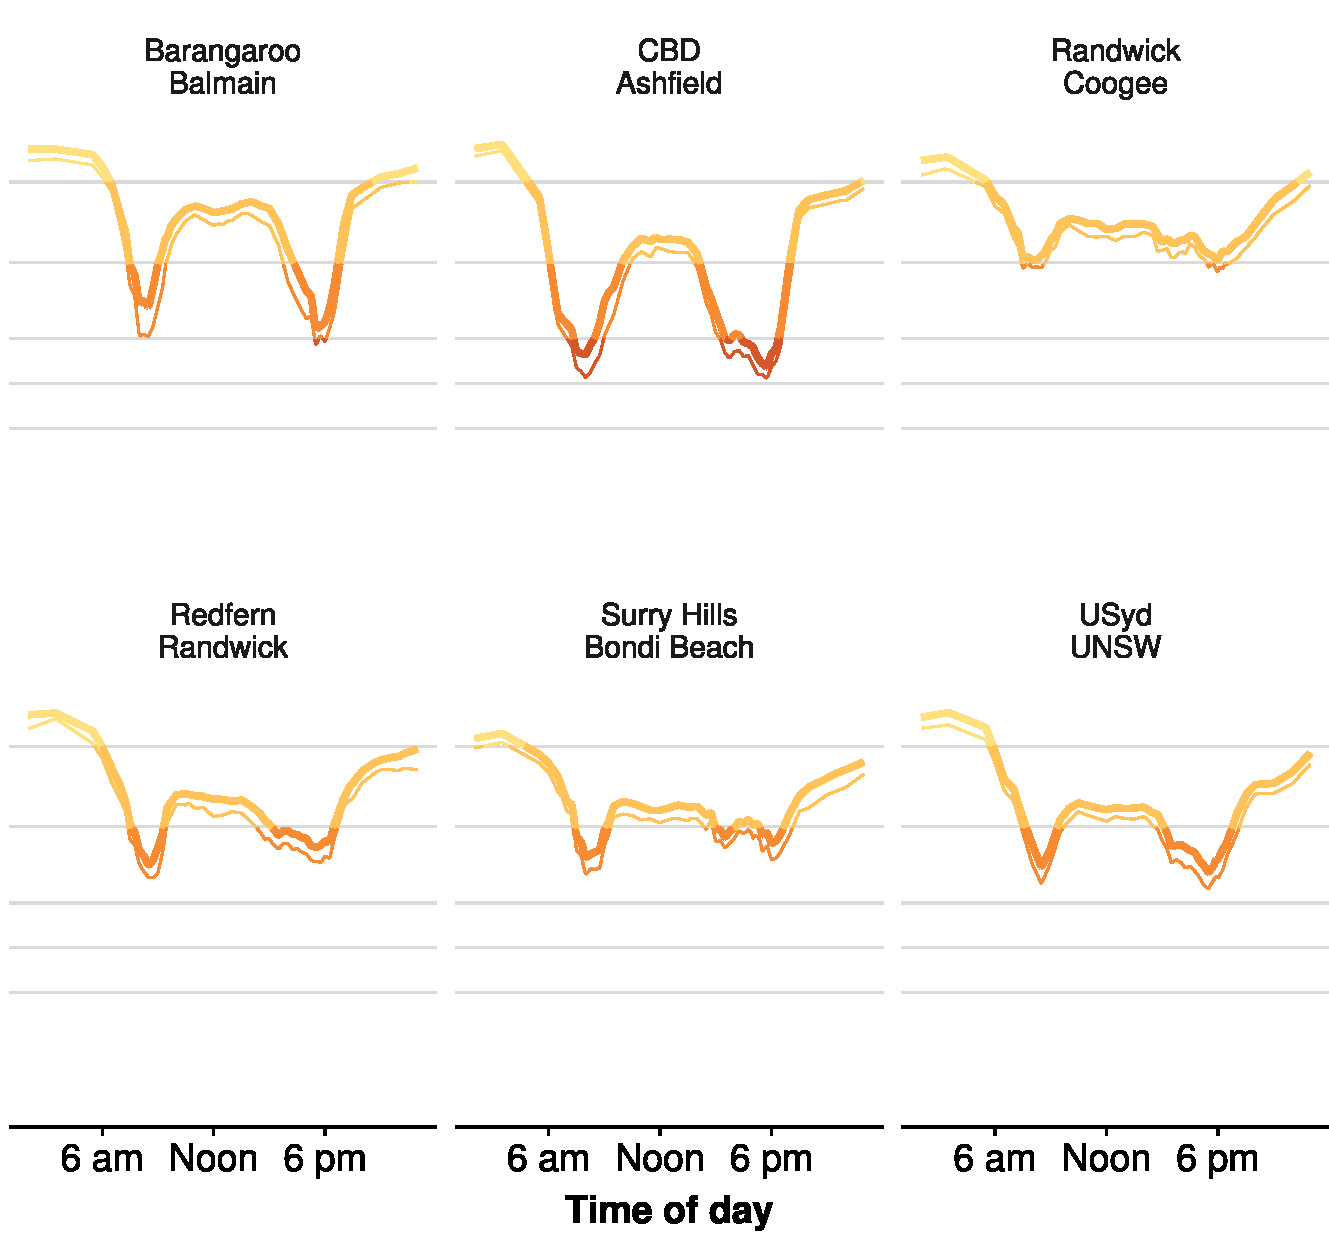
\includegraphics{atlas/Avg-LOS-short-routes-SYD-1.pdf}
  \null\vfill\null
\end{minipage}
\end{figure*}

Urban freeways appear to offer less stable traffic flows, at least in some locations. Average speeds on Melbourne's inner-suburban freeways (which typically have speed limits of 80 kilometres per hour) have fallen below 50 kilometres per hour during the morning peak period since 2010 (see \Vref{fig:speed-Vic-freeways-vs-year}). Melbourne's middle and outer-region urban freeways appear to have much more stable traffic flows,%
    \footcite{Vicroads-201415-TravelSpeed-tableau}
but time-of-day analysis is not possible (nor pubilcly available) for urban freeways.%
    \footnote{Our data is not well suited to assessing the level of service on freeways, because it requires the use of precise postal addresses as origins and destinations, which is not possible to do for freeway segments.}



\section{A path through -- how to identify excessive congestion?}\label{tbl:a-path-through}

This chapter and the previous chapter have shown that how bad you think congestion is depends on your perspective, and how costly you think it is depends on how you measure the costs. Each is based on sound principles and contributes to an understanding of congestion, but each also has its drawbacks. 

\begin{itemize}
\item The motorists’ perspective lacks grounding without the backing of some theory that explains why certain levels of delay are problematic. 
\item The engineering view provides a clear perspective on the efficiency of roads, but few motorists or economists would agree that roads that have travel speeds falling to below half of the free-flow speed is an acceptable outcome for the economic and the “liveability” performance of a city – even if the total vehicle flow is still increasing. 
\item The economists view is theoretically sound, but very difficult to measure with any precision. 
\end{itemize}

From this, the challenges for precisely identifying “excessive congestion” are clear. 
But it is possible to get a clear sense of “excessive” by combining the principle of the economists’ perspective – that delays are costly, and arise because motorists do not consider the full costs of their travel decisions – and combine this view with measures of delay and variability from the motorist view. Adopting this perspective allows us to see that, in some places and at certain times of day, congestion is a problem that governments should be actively trying to counter.

To understand how we can do that in Sydney and Melbourne, a more ``micro-level" analysis of each city is required; an examination of the magnitude of congestion in different parts of the city at different times of the day and week.



\appendix
\chapter{Defining congestion}\label{chap:appendix-defining-congestion}

Roads are “congested” when the number of vehicles using them causes unacceptable levels of discomfort and delay.%
    \footcite[][93]{Falcocchio-and-Levinson-congestion-a-concise-guide}
But of course “unacceptable” means different things to different people. Three different perspectives – those of motorists, engineers, and economists -- provide definitions that can help policy-makers.%
    \footcite[][7]{Wallis-Lupton-2013-NZ-Transport-Agency}

Motorists see aggravation.
Economists see costs.
But engineers tend to say that, most of the time and in most locations, we are not short of physical capacity on our roads -- so what's the problem?

\phantomsection
\label{para:three-perspectives-on-congestion--intro}
\zlabel{para:three-perspectives-on-congestion--intro}
The three perspectives are set out below.

\section{Motorists care about travel time and reliability}\label{subsec:road-users-perspective}
For motorists, a road is too congested if their speeds drop too far and their trip takes too much longer than expected. Expected travel time is subjective, and depends on location, time of day, and type of road. The motorist's perspective is sometimes referred to as “perceived” congestion.%
    \footcite[][108]{Falcocchio-and-Levinson-congestion-a-concise-guide}

The main way to assess congestion from the motorist's perspective is to compare travel times when there is congestion with travel times for the same trip when there is no congestion – usually in the middle of the night.

This measure is useful for policy-makers only when comparing congestion across cities of similar sizes.
This is because the economic cost of congestion depends on the size of the city.
If a trip takes 50 per cent longer in peak hour than it would in the middle of the night, the economic costs it imposes will be larger in a city that has longer average trip lengths and more people taking the trip – \ie~in larger cities.

So comparing Sydney with Melbourne is much more useful than comparing Sydney with, say, Canberra.

\section{Engineers care about a road's physical capacity}\label{subsec:engineers-perspective}
Traffic engineers consider a road congested when more vehicles are attempting to use the road than it has physical capacity to carry.%
    \footcite[][7]{Wallis-Lupton-2013-NZ-Transport-Agency}
Capacity refers to the maximum number of vehicles the road is capable of carrying over a fixed period – the maximum possible throughput.

When traffic flows are moderate, more vehicles can enter the stream of traffic and the overall throughput of the road can keep increasing.
But there comes a point where more vehicles entering the stream of traffic leads to a crop in overall throughput: when individual vehicles slow down to deal with all the other vehicles braking, changing lane and sharing the road space.

\begin{figureTop}
\caption{Optimal traffic levels depend on the relationship between throughput, density and speed \label{fig:Arnott-flow-curves}}
\units{Traffic throughput (\eg~vehicles per hour), density (\eg~vehicles per 100 meters of road) and speed (\eg~km\,/\,h)}
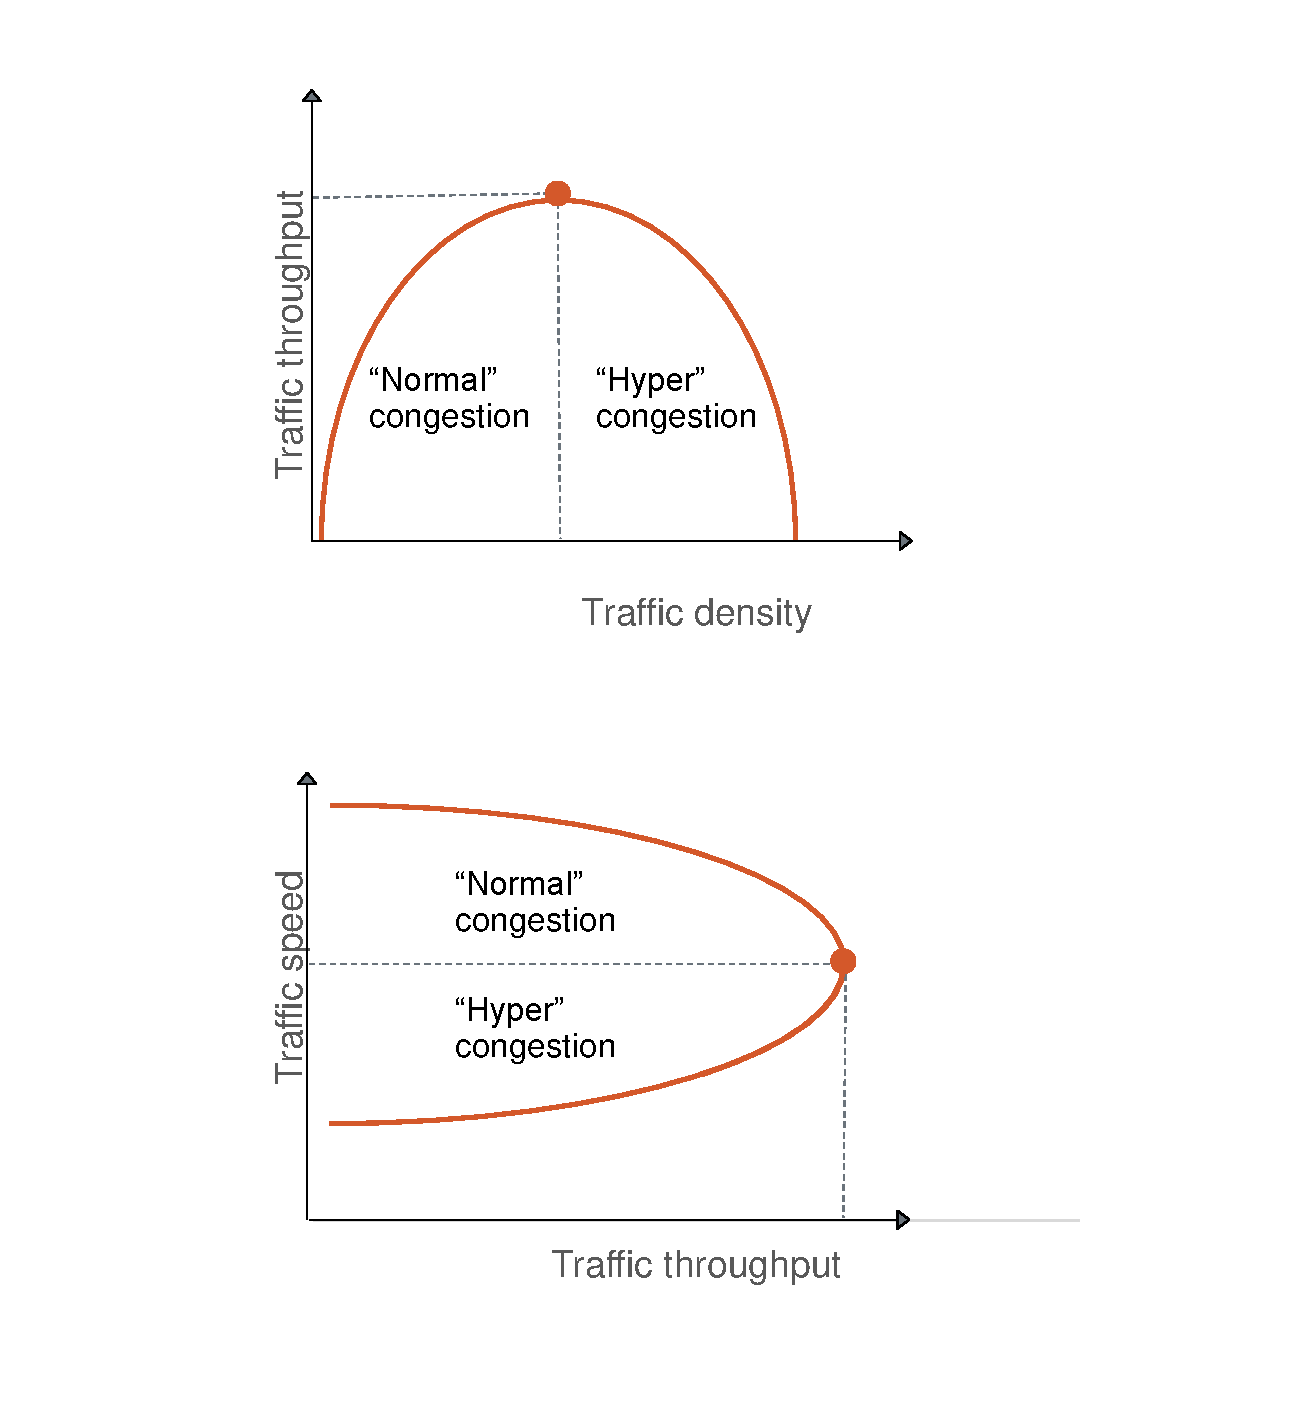
\includegraphics[page=1]{Charts/ChartPackLong.pdf}
\noteswithsource{These curves present the theoretical relationship between these variables. \textcite{Chavis-etal-2011-Multimodal-transport-Nairobi} provide empirical evidence for this relationship using data from a range of cities internationally.}{\textcites[][29]{Arnott-2015-Bathtub-model-of-traffic-congestion}{Austroads-2015-Guide-Traffic-Mgmt}}
\end{figureTop}

The first curve in \Vref{fig:Arnott-flow-curves} shows traffic throughput initially increasing with greater traffic density, but eventually decreasing as the number of vehicles on the road becomes too high.

The second curve in \Cref{fig:Arnott-flow-curves} tells a similar story.
Reading the curve clockwise, speed gradually falls as traffic density increases.
But throughout continues to increase up to a certain point (the ``bullet nose'' of the curve), after which speed and throughput both decline.

The first half of each curve in \Cref{fig:Arnott-flow-curves} shows “normal” congestion.
The second half shows ``hyper'' congestion: the road is being used beyond its capacity.

Each time a vehicle joins a road, it slows everyone else.
This can impose a cost on the other motorists, even before the road becomes hyper-congested.
The following section focuses on this way of viewing congestion.


\section{Economists care about how the value of trips compares with the costs those trips impose on everyone} \label{subsec:Economists-perspective}

Economists focus on the costs and benefits that road users experience at different levels of traffic flow.
They pay particular attention to the difference between the private cost of an additional trip and the social cost of that trip.

\begin{itemize}
\item The private cost is incurred by the person who takes the trip, and includes tolls, the cost of fuel, the cost of wear and tear on a car and the value to the person of the time taken to make the trip.
\item The social cost is the private cost \textbf{plus} the cost that the trip may impose on \textbf{others}, mainly in the form of the time added to the trips of every other road user.%
\footnote{The social cost excludes any tolls, because they are transfers to another party.
As well as congestion, social costs include pollution and accidents.}
\end{itemize}

\begin{bigbox}{What do economists really mean by when they talk about the social costs of driving?}{box:explaining-congestion-as-negative-externality}

When economists refer to the social costs of driving (see \Cref{subsec:Economists-perspective}) they are pointing to costs beyond those borne by the individual driver.
When a driver decides to take a trip, after weighing up the private costs and benefits of that trip, the broader community can pay a price through congestion.

To understand this better, let's think about a particular situation.

Imagine a person who commutes from home to work each weekday.
During the morning peak, her trip takes around 60 minutes.
So she knows that to reach the office by 9\,am she needs to be in the car by 8\,am.

For simplicity, let's assume the entire trip is on a freeway, and there is a single set of traffic lights at the end of the freeway at which motorists regularly spend 30 minutes waiting to get through on any given morning.

Why would she do it? Clearly, when she thinks about the costs and benefits of travelling by car versus alternatives such as travelling by train or driving  earlier in the morning before the rush, the benefits outweigh the costs.
But while the benefits might outweigh \textit{her} costs, economists emphasise the costs she imposes on other motorists by making congestion that little bit worse.

The best way to see these congestion costs is to imagine removing her trip.
If she was at the front of the traffic-light queue, removing her from the stream of traffic makes it possible for a car that would otherwise have had to wait for another light cycle to make it through.
If the light cycle takes one minute, then removing her one vehicle has reduced congestion by one-minute for one other motorist.

But the impact doesn't end there – with the line of cars now one fewer than it was before, at the following light change it is again possible for an additional driver to make it through, saving one more minute for one more motorist.
The time savings will continue for as long as the congestion lasts.
If the original motorist is removed when there is one-hour of congestion left, then there is a saving of 30 minutes of time for other drivers – one minute at 30 changes of lights (if we assume that the lights go red for one minute, and green for the next minute).

Our motorist might think of herself as “just one more car”, but the costs she imposes on other drivers are significant.
If we value people's time at \$20 an hour, just those 30 minutes has imposed additional “social” costs of \$10 that were not considered when the original private travel decision was made.

If this trip is assumed to be representative of all trips, then a rough rule of thumb for the economic costs of congestion would be to multiply the \$10 estimated social cost of a trip by the total number of trips during the morning peak.
The economists' point is clear: the costs individual motorists impose on the broader community, and which they often do not even consider, are likely to be large.

\boxsources{\textcite{King-and-Gans-Finishing-the-Job}}
\end{bigbox}

Economists will see ``excessive'' congestion well before engineers do; it is not hard to imagine that, when a road is busy, the social cost of a trip may be much higher than the private cost of a trip (\Vref{box:explaining-congestion-as-negative-externality}).

\phantomsection
\label{para:three-perspectives-on-congestion--end}

